\documentclass[1p]{elsarticle_modified}
%\bibliographystyle{elsarticle-num}

%\usepackage[colorlinks]{hyperref}
%\usepackage{abbrmath_seonhwa} %\Abb, \Ascr, \Acal ,\Abf, \Afrak
\usepackage{amsfonts}
\usepackage{amssymb}
\usepackage{amsmath}
\usepackage{amsthm}
\usepackage{scalefnt}
\usepackage{amsbsy}
\usepackage{kotex}
\usepackage{caption}
\usepackage{subfig}
\usepackage{color}
\usepackage{graphicx}
\usepackage{xcolor} %% white, black, red, green, blue, cyan, magenta, yellow
\usepackage{float}
\usepackage{setspace}
\usepackage{hyperref}

\usepackage{tikz}
\usetikzlibrary{arrows}

\usepackage{multirow}
\usepackage{array} % fixed length table
\usepackage{hhline}

%%%%%%%%%%%%%%%%%%%%%
\makeatletter
\renewcommand*\env@matrix[1][\arraystretch]{%
	\edef\arraystretch{#1}%
	\hskip -\arraycolsep
	\let\@ifnextchar\new@ifnextchar
	\array{*\c@MaxMatrixCols c}}
\makeatother %https://tex.stackexchange.com/questions/14071/how-can-i-increase-the-line-spacing-in-a-matrix
%%%%%%%%%%%%%%%

\usepackage[normalem]{ulem}

\newcommand{\msout}[1]{\ifmmode\text{\sout{\ensuremath{#1}}}\else\sout{#1}\fi}
%SOURCE: \msout is \stkout macro in https://tex.stackexchange.com/questions/20609/strikeout-in-math-mode

\newcommand{\cancel}[1]{
	\ifmmode
	{\color{red}\msout{#1}}
	\else
	{\color{red}\sout{#1}}
	\fi
}

\newcommand{\add}[1]{
	{\color{blue}\uwave{#1}}
}

\newcommand{\replace}[2]{
	\ifmmode
	{\color{red}\msout{#1}}{\color{blue}\uwave{#2}}
	\else
	{\color{red}\sout{#1}}{\color{blue}\uwave{#2}}
	\fi
}

\newcommand{\Sol}{\mathcal{S}} %segment
\newcommand{\D}{D} %diagram
\newcommand{\A}{\mathcal{A}} %arc


%%%%%%%%%%%%%%%%%%%%%%%%%%%%%5 test

\def\sl{\operatorname{\textup{SL}}(2,\Cbb)}
\def\psl{\operatorname{\textup{PSL}}(2,\Cbb)}
\def\quan{\mkern 1mu \triangleright \mkern 1mu}

\theoremstyle{definition}
\newtheorem{thm}{Theorem}[section]
\newtheorem{prop}[thm]{Proposition}
\newtheorem{lem}[thm]{Lemma}
\newtheorem{ques}[thm]{Question}
\newtheorem{cor}[thm]{Corollary}
\newtheorem{defn}[thm]{Definition}
\newtheorem{exam}[thm]{Example}
\newtheorem{rmk}[thm]{Remark}
\newtheorem{alg}[thm]{Algorithm}

\newcommand{\I}{\sqrt{-1}}
\begin{document}

%\begin{frontmatter}
%
%\title{Boundary parabolic representations of knots up to 8 crossings}
%
%%% Group authors per affiliation:
%\author{Yunhi Cho} 
%\address{Department of Mathematics, University of Seoul, Seoul, Korea}
%\ead{yhcho@uos.ac.kr}
%
%
%\author{Seonhwa Kim} %\fnref{s_kim}}
%\address{Center for Geometry and Physics, Institute for Basic Science, Pohang, 37673, Korea}
%\ead{ryeona17@ibs.re.kr}
%
%\author{Hyuk Kim}
%\address{Department of Mathematical Sciences, Seoul National University, Seoul 08826, Korea}
%\ead{hyukkim@snu.ac.kr}
%
%\author{Seokbeom Yoon}
%\address{Department of Mathematical Sciences, Seoul National University, Seoul, 08826,  Korea}
%\ead{sbyoon15@snu.ac.kr}
%
%\begin{abstract}
%We find all boundary parabolic representation of knots up to 8 crossings.
%
%\end{abstract}
%\begin{keyword}
%    \MSC[2010] 57M25 
%\end{keyword}
%
%\end{frontmatter}

%\linenumbers
%\tableofcontents
%
\newcommand\colored[1]{\textcolor{white}{\rule[-0.35ex]{0.8em}{1.4ex}}\kern-0.8em\color{red} #1}%
%\newcommand\colored[1]{\textcolor{white}{ #1}\kern-2.17ex	\textcolor{white}{ #1}\kern-1.81ex	\textcolor{white}{ #1}\kern-2.15ex\color{red}#1	}

{\Large $\underline{12a_{0300}~(K12a_{0300})}$}

\setlength{\tabcolsep}{10pt}
\renewcommand{\arraystretch}{1.6}
\vspace{1cm}\begin{tabular}{m{100pt}>{\centering\arraybackslash}m{274pt}}
\multirow{5}{120pt}{
	\centering
	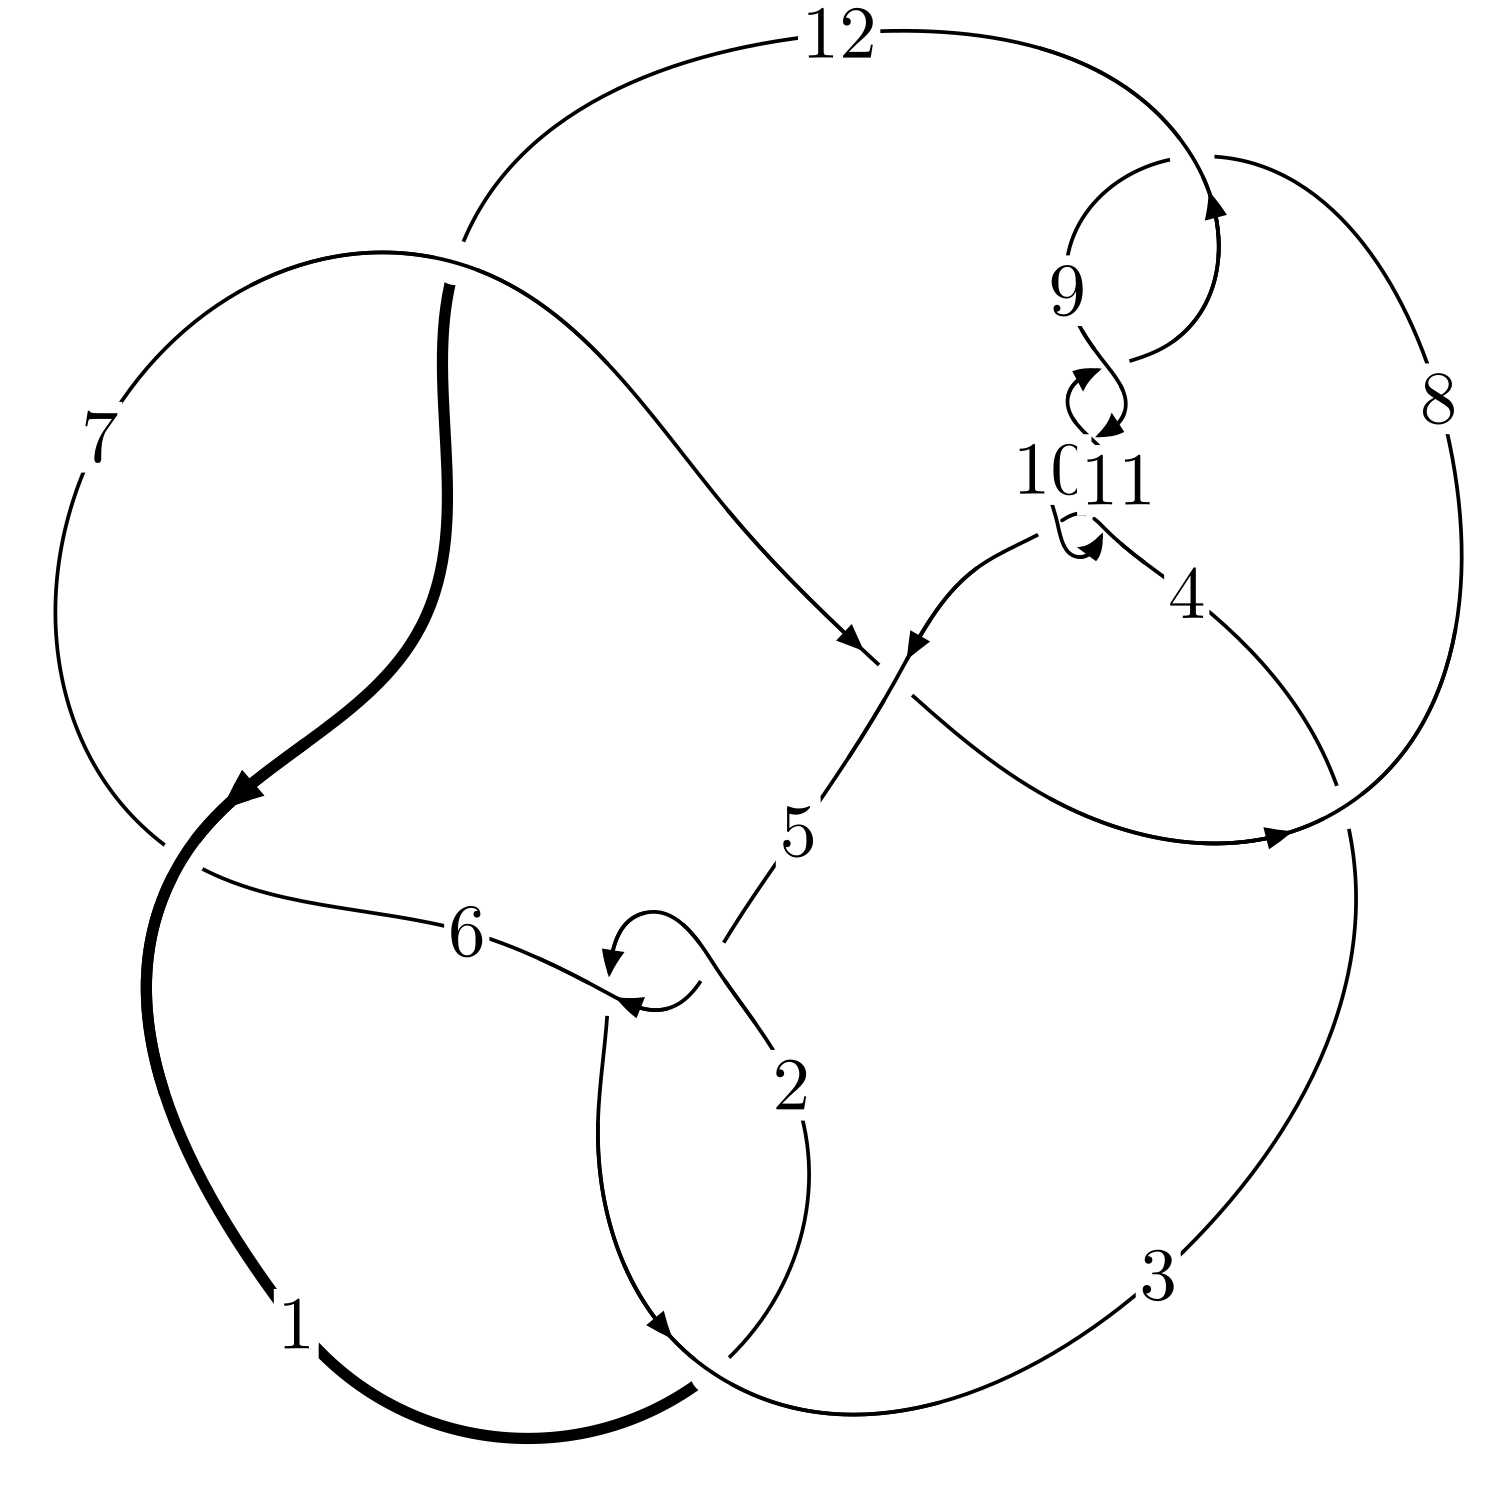
\includegraphics[width=112pt]{../../../GIT/diagram.site/Diagrams/png/1101_12a_0300.png}\\
\ \ \ A knot diagram\footnotemark}&
\allowdisplaybreaks
\textbf{Linearized knot diagam} \\
\cline{2-2}
 &
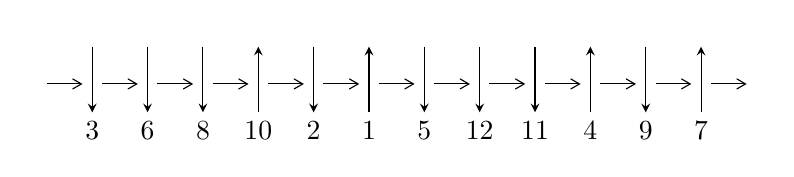
\begin{tikzpicture}[x=20pt, y=17pt]
	% nodes
	\node (C0) at (0, 0) {};
	\node (C1) at (1, 0) {};
	\node (C1U) at (1, +1) {};
	\node (C1D) at (1, -1) {3};

	\node (C2) at (2, 0) {};
	\node (C2U) at (2, +1) {};
	\node (C2D) at (2, -1) {6};

	\node (C3) at (3, 0) {};
	\node (C3U) at (3, +1) {};
	\node (C3D) at (3, -1) {8};

	\node (C4) at (4, 0) {};
	\node (C4U) at (4, +1) {};
	\node (C4D) at (4, -1) {10};

	\node (C5) at (5, 0) {};
	\node (C5U) at (5, +1) {};
	\node (C5D) at (5, -1) {2};

	\node (C6) at (6, 0) {};
	\node (C6U) at (6, +1) {};
	\node (C6D) at (6, -1) {1};

	\node (C7) at (7, 0) {};
	\node (C7U) at (7, +1) {};
	\node (C7D) at (7, -1) {5};

	\node (C8) at (8, 0) {};
	\node (C8U) at (8, +1) {};
	\node (C8D) at (8, -1) {12};

	\node (C9) at (9, 0) {};
	\node (C9U) at (9, +1) {};
	\node (C9D) at (9, -1) {11};

	\node (C10) at (10, 0) {};
	\node (C10U) at (10, +1) {};
	\node (C10D) at (10, -1) {4};

	\node (C11) at (11, 0) {};
	\node (C11U) at (11, +1) {};
	\node (C11D) at (11, -1) {9};

	\node (C12) at (12, 0) {};
	\node (C12U) at (12, +1) {};
	\node (C12D) at (12, -1) {7};
	\node (C13) at (13, 0) {};

	% arrows
	\draw[->,>={angle 60}]
	(C0) edge (C1) (C1) edge (C2) (C2) edge (C3) (C3) edge (C4) (C4) edge (C5) (C5) edge (C6) (C6) edge (C7) (C7) edge (C8) (C8) edge (C9) (C9) edge (C10) (C10) edge (C11) (C11) edge (C12) (C12) edge (C13) ;	\draw[->,>=stealth]
	(C1U) edge (C1D) (C2U) edge (C2D) (C3U) edge (C3D) (C4D) edge (C4U) (C5U) edge (C5D) (C6D) edge (C6U) (C7U) edge (C7D) (C8U) edge (C8D) (C9U) edge (C9D) (C10D) edge (C10U) (C11U) edge (C11D) (C12D) edge (C12U) ;
	\end{tikzpicture} \\
\hhline{~~} \\& 
\textbf{Solving Sequence} \\ \cline{2-2} 
 &
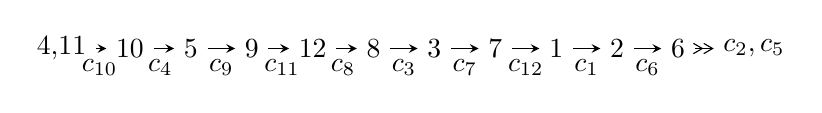
\begin{tikzpicture}[x=22pt, y=7pt]
	% node
	\node (A0) at (-1/8, 0) {4,11};
	\node (A1) at (1, 0) {10};
	\node (A2) at (2, 0) {5};
	\node (A3) at (3, 0) {9};
	\node (A4) at (4, 0) {12};
	\node (A5) at (5, 0) {8};
	\node (A6) at (6, 0) {3};
	\node (A7) at (7, 0) {7};
	\node (A8) at (8, 0) {1};
	\node (A9) at (9, 0) {2};
	\node (A10) at (10, 0) {6};
	\node (C1) at (1/2, -1) {$c_{10}$};
	\node (C2) at (3/2, -1) {$c_{4}$};
	\node (C3) at (5/2, -1) {$c_{9}$};
	\node (C4) at (7/2, -1) {$c_{11}$};
	\node (C5) at (9/2, -1) {$c_{8}$};
	\node (C6) at (11/2, -1) {$c_{3}$};
	\node (C7) at (13/2, -1) {$c_{7}$};
	\node (C8) at (15/2, -1) {$c_{12}$};
	\node (C9) at (17/2, -1) {$c_{1}$};
	\node (C10) at (19/2, -1) {$c_{6}$};
	\node (A11) at (45/4, 0) {$c_{2},c_{5}$};

	% edge
	\draw[->,>=stealth]	
	(A0) edge (A1) (A1) edge (A2) (A2) edge (A3) (A3) edge (A4) (A4) edge (A5) (A5) edge (A6) (A6) edge (A7) (A7) edge (A8) (A8) edge (A9) (A9) edge (A10) ;
	\draw[->>,>={angle 60}]	
	(A10) edge (A11);
\end{tikzpicture} \\ 

\end{tabular} \\

\footnotetext{
The image of knot diagram is generated by the software ``\textbf{Draw programme}" developed by Andrew Bartholomew(\url{http://www.layer8.co.uk/maths/draw/index.htm\#Running-draw}), where we modified some parts for our purpose(\url{https://github.com/CATsTAILs/LinksPainter}).
}\phantom \\ \newline 
\centering \textbf{Ideals for irreducible components\footnotemark of $X_{\text{par}}$} 
 
\begin{align*}
I^u_{1}&=\langle 
u^{77}+u^{76}+\cdots+u+1\rangle \\
\\
\end{align*}
\raggedright * 1 irreducible components of $\dim_{\mathbb{C}}=0$, with total 77 representations.\\
\footnotetext{All coefficients of polynomials are rational numbers. But the coefficients are sometimes approximated in decimal forms when there is not enough margin.}
\newpage
\renewcommand{\arraystretch}{1}
\centering \section*{I. $I^u_{1}= \langle u^{77}+u^{76}+\cdots+u+1 \rangle$}
\flushleft \textbf{(i) Arc colorings}\\
\begin{tabular}{m{7pt} m{180pt} m{7pt} m{180pt} }
\flushright $a_{4}=$&$\begin{pmatrix}0\\u\end{pmatrix}$ \\
\flushright $a_{11}=$&$\begin{pmatrix}1\\0\end{pmatrix}$ \\
\flushright $a_{10}=$&$\begin{pmatrix}1\\u^2\end{pmatrix}$ \\
\flushright $a_{5}=$&$\begin{pmatrix}u\\u^3+u\end{pmatrix}$ \\
\flushright $a_{9}=$&$\begin{pmatrix}u^2+1\\u^2\end{pmatrix}$ \\
\flushright $a_{12}=$&$\begin{pmatrix}u^4+u^2+1\\u^4\end{pmatrix}$ \\
\flushright $a_{8}=$&$\begin{pmatrix}u^6+u^4+2 u^2+1\\u^6+u^2\end{pmatrix}$ \\
\flushright $a_{3}=$&$\begin{pmatrix}u^{13}+2 u^{11}+5 u^9+6 u^7+6 u^5+4 u^3+u\\u^{13}+u^{11}+3 u^9+2 u^7+2 u^5+u^3+u\end{pmatrix}$ \\
\flushright $a_{7}=$&$\begin{pmatrix}- u^{10}- u^8-2 u^6- u^4+u^2+1\\- u^{12}-2 u^{10}-4 u^8-4 u^6-3 u^4\end{pmatrix}$ \\
\flushright $a_{1}=$&$\begin{pmatrix}- u^{26}-3 u^{24}+\cdots+u^2+1\\- u^{28}-4 u^{26}+\cdots-12 u^8+u^4\end{pmatrix}$ \\
\flushright $a_{2}=$&$\begin{pmatrix}u^{54}+7 u^{52}+\cdots+2 u^2+1\\u^{54}+6 u^{52}+\cdots+4 u^4+u^2\end{pmatrix}$ \\
\flushright $a_{6}=$&$\begin{pmatrix}- u^{42}-5 u^{40}+\cdots+u^2+1\\- u^{44}-6 u^{42}+\cdots-4 u^6-3 u^4\end{pmatrix}$\\&\end{tabular}
\flushleft \textbf{(ii) Obstruction class $= -1$}\\~\\
\flushleft \textbf{(iii) Cusp Shapes $= -4 u^{75}-4 u^{74}+\cdots-4 u-6$}\\~\\
\newpage\renewcommand{\arraystretch}{1}
\flushleft \textbf{(iv) u-Polynomials at the component}\newline \\
\begin{tabular}{m{50pt}|m{274pt}}
Crossings & \hspace{64pt}u-Polynomials at each crossing \\
\hline $$\begin{aligned}c_{1}\end{aligned}$$&$\begin{aligned}
&u^{77}+41 u^{76}+\cdots- u+1
\end{aligned}$\\
\hline $$\begin{aligned}c_{2},c_{5}\end{aligned}$$&$\begin{aligned}
&u^{77}+u^{76}+\cdots+3 u+1
\end{aligned}$\\
\hline $$\begin{aligned}c_{3}\end{aligned}$$&$\begin{aligned}
&u^{77}+u^{76}+\cdots-3 u+1
\end{aligned}$\\
\hline $$\begin{aligned}c_{4},c_{10}\end{aligned}$$&$\begin{aligned}
&u^{77}+u^{76}+\cdots+u+1
\end{aligned}$\\
\hline $$\begin{aligned}c_{6},c_{12}\end{aligned}$$&$\begin{aligned}
&u^{77}+3 u^{76}+\cdots+15 u+3
\end{aligned}$\\
\hline $$\begin{aligned}c_{7}\end{aligned}$$&$\begin{aligned}
&u^{77}-9 u^{76}+\cdots-303 u+29
\end{aligned}$\\
\hline $$\begin{aligned}c_{8},c_{9},c_{11}\end{aligned}$$&$\begin{aligned}
&u^{77}+19 u^{76}+\cdots- u-1
\end{aligned}$\\
\hline
\end{tabular}\\~\\
\newpage\renewcommand{\arraystretch}{1}
\flushleft \textbf{(v) Riley Polynomials at the component}\newline \\
\begin{tabular}{m{50pt}|m{274pt}}
Crossings & \hspace{64pt}Riley Polynomials at each crossing \\
\hline $$\begin{aligned}c_{1}\end{aligned}$$&$\begin{aligned}
&y^{77}-9 y^{76}+\cdots- y-1
\end{aligned}$\\
\hline $$\begin{aligned}c_{2},c_{5}\end{aligned}$$&$\begin{aligned}
&y^{77}-41 y^{76}+\cdots- y-1
\end{aligned}$\\
\hline $$\begin{aligned}c_{3}\end{aligned}$$&$\begin{aligned}
&y^{77}- y^{76}+\cdots-193 y-1
\end{aligned}$\\
\hline $$\begin{aligned}c_{4},c_{10}\end{aligned}$$&$\begin{aligned}
&y^{77}+19 y^{76}+\cdots- y-1
\end{aligned}$\\
\hline $$\begin{aligned}c_{6},c_{12}\end{aligned}$$&$\begin{aligned}
&y^{77}+59 y^{76}+\cdots-1401 y-9
\end{aligned}$\\
\hline $$\begin{aligned}c_{7}\end{aligned}$$&$\begin{aligned}
&y^{77}+11 y^{76}+\cdots+15191 y-841
\end{aligned}$\\
\hline $$\begin{aligned}c_{8},c_{9},c_{11}\end{aligned}$$&$\begin{aligned}
&y^{77}+79 y^{76}+\cdots+7 y-1
\end{aligned}$\\
\hline
\end{tabular}\\~\\
\newpage\flushleft \textbf{(vi) Complex Volumes and Cusp Shapes}
$$\begin{array}{c|c|c}  
\text{Solutions to }I^u_{1}& \I (\text{vol} + \sqrt{-1}CS) & \text{Cusp shape}\\
 \hline 
\begin{aligned}
u &= -0.384157 + 0.916651 I\end{aligned}
 & -0.08016 - 6.28454 I & \phantom{-0.000000 -}0. + 10.45893 I \\ \hline\begin{aligned}
u &= -0.384157 - 0.916651 I\end{aligned}
 & -0.08016 + 6.28454 I & \phantom{-0.000000 } 0. - 10.45893 I \\ \hline\begin{aligned}
u &= -0.359432 + 0.963246 I\end{aligned}
 & -3.28646 - 6.49921 I & \phantom{-0.000000 } 0 \\ \hline\begin{aligned}
u &= -0.359432 - 0.963246 I\end{aligned}
 & -3.28646 + 6.49921 I & \phantom{-0.000000 } 0 \\ \hline\begin{aligned}
u &= \phantom{-}0.181375 + 0.954789 I\end{aligned}
 & -8.18742 + 3.05866 I & -13.52379 - 3.93661 I \\ \hline\begin{aligned}
u &= \phantom{-}0.181375 - 0.954789 I\end{aligned}
 & -8.18742 - 3.05866 I & -13.52379 + 3.93661 I \\ \hline\begin{aligned}
u &= \phantom{-}0.344445 + 0.969057 I\end{aligned}
 & -7.25591 + 2.51870 I & \phantom{-0.000000 } 0 \\ \hline\begin{aligned}
u &= \phantom{-}0.344445 - 0.969057 I\end{aligned}
 & -7.25591 - 2.51870 I & \phantom{-0.000000 } 0 \\ \hline\begin{aligned}
u &= \phantom{-}0.151839 + 0.956150 I\end{aligned}
 & -7.61091 - 5.67836 I & -12.50459 + 3.10607 I \\ \hline\begin{aligned}
u &= \phantom{-}0.151839 - 0.956150 I\end{aligned}
 & -7.61091 + 5.67836 I & -12.50459 - 3.10607 I \\ \hline\begin{aligned}
u &= \phantom{-}0.364368 + 0.973455 I\end{aligned}
 & -6.39842 + 11.27770 I & \phantom{-0.000000 } 0 \\ \hline\begin{aligned}
u &= \phantom{-}0.364368 - 0.973455 I\end{aligned}
 & -6.39842 - 11.27770 I & \phantom{-0.000000 } 0 \\ \hline\begin{aligned}
u &= \phantom{-}0.387418 + 0.873983 I\end{aligned}
 & \phantom{-}0.51259 + 2.09295 I & -1.92214 - 3.70673 I \\ \hline\begin{aligned}
u &= \phantom{-}0.387418 - 0.873983 I\end{aligned}
 & \phantom{-}0.51259 - 2.09295 I & -1.92214 + 3.70673 I \\ \hline\begin{aligned}
u &= -0.162879 + 0.940953 I\end{aligned}
 & -4.40542 + 1.03814 I & -9.57563 + 0. I\phantom{ +0.000000I} \\ \hline\begin{aligned}
u &= -0.162879 - 0.940953 I\end{aligned}
 & -4.40542 - 1.03814 I & -9.57563 + 0. I\phantom{ +0.000000I} \\ \hline\begin{aligned}
u &= -0.279119 + 0.907947 I\end{aligned}
 & -3.80142 - 2.48917 I & -13.3851 + 5.1983 I \\ \hline\begin{aligned}
u &= -0.279119 - 0.907947 I\end{aligned}
 & -3.80142 + 2.48917 I & -13.3851 - 5.1983 I \\ \hline\begin{aligned}
u &= -0.735571 + 0.878240 I\end{aligned}
 & -2.84182 + 1.57464 I & \phantom{-0.000000 } 0 \\ \hline\begin{aligned}
u &= -0.735571 - 0.878240 I\end{aligned}
 & -2.84182 - 1.57464 I & \phantom{-0.000000 } 0 \\ \hline\begin{aligned}
u &= -0.529170 + 0.664612 I\end{aligned}
 & -3.03277 + 2.04853 I & -4.86577 + 0.18647 I \\ \hline\begin{aligned}
u &= -0.529170 - 0.664612 I\end{aligned}
 & -3.03277 - 2.04853 I & -4.86577 - 0.18647 I \\ \hline\begin{aligned}
u &= -0.099359 + 0.832534 I\end{aligned}
 & -1.57015 + 1.62706 I & -8.90717 - 3.48380 I \\ \hline\begin{aligned}
u &= -0.099359 - 0.832534 I\end{aligned}
 & -1.57015 - 1.62706 I & -8.90717 + 3.48380 I \\ \hline\begin{aligned}
u &= \phantom{-}0.328773 + 0.768032 I\end{aligned}
 & -0.30487 + 1.47590 I & -2.27756 - 4.79967 I \\ \hline\begin{aligned}
u &= \phantom{-}0.328773 - 0.768032 I\end{aligned}
 & -0.30487 - 1.47590 I & -2.27756 + 4.79967 I \\ \hline\begin{aligned}
u &= \phantom{-}0.752498 + 0.891905 I\end{aligned}
 & \phantom{-}0.60818 + 2.85389 I & \phantom{-0.000000 } 0 \\ \hline\begin{aligned}
u &= \phantom{-}0.752498 - 0.891905 I\end{aligned}
 & \phantom{-}0.60818 - 2.85389 I & \phantom{-0.000000 } 0 \\ \hline\begin{aligned}
u &= -0.743580 + 0.908600 I\end{aligned}
 & -2.94895 - 7.20020 I & \phantom{-0.000000 } 0 \\ \hline\begin{aligned}
u &= -0.743580 - 0.908600 I\end{aligned}
 & -2.94895 + 7.20020 I & \phantom{-0.000000 } 0\\
 \hline 
 \end{array}$$\newpage$$\begin{array}{c|c|c}  
\text{Solutions to }I^u_{1}& \I (\text{vol} + \sqrt{-1}CS) & \text{Cusp shape}\\
 \hline 
\begin{aligned}
u &= \phantom{-}0.829686 + 0.851767 I\end{aligned}
 & \phantom{-}3.00542 + 0.05293 I & \phantom{-0.000000 } 0 \\ \hline\begin{aligned}
u &= \phantom{-}0.829686 - 0.851767 I\end{aligned}
 & \phantom{-}3.00542 - 0.05293 I & \phantom{-0.000000 } 0 \\ \hline\begin{aligned}
u &= -0.866902 + 0.822657 I\end{aligned}
 & \phantom{-}0.526126 + 0.450966 I & \phantom{-0.000000 } 0 \\ \hline\begin{aligned}
u &= -0.866902 - 0.822657 I\end{aligned}
 & \phantom{-}0.526126 - 0.450966 I & \phantom{-0.000000 } 0 \\ \hline\begin{aligned}
u &= -0.571449 + 0.558788 I\end{aligned}
 & -2.66165 - 6.09408 I & -3.39785 + 6.85504 I \\ \hline\begin{aligned}
u &= -0.571449 - 0.558788 I\end{aligned}
 & -2.66165 + 6.09408 I & -3.39785 - 6.85504 I \\ \hline\begin{aligned}
u &= \phantom{-}0.872860 + 0.828358 I\end{aligned}
 & \phantom{-}4.63295 - 4.30393 I & \phantom{-0.000000 } 0 \\ \hline\begin{aligned}
u &= \phantom{-}0.872860 - 0.828358 I\end{aligned}
 & \phantom{-}4.63295 + 4.30393 I & \phantom{-0.000000 } 0 \\ \hline\begin{aligned}
u &= -0.877082 + 0.825271 I\end{aligned}
 & \phantom{-}1.61683 + 9.16430 I & \phantom{-0.000000 } 0 \\ \hline\begin{aligned}
u &= -0.877082 - 0.825271 I\end{aligned}
 & \phantom{-}1.61683 - 9.16430 I & \phantom{-0.000000 } 0 \\ \hline\begin{aligned}
u &= \phantom{-}0.871205 + 0.847546 I\end{aligned}
 & \phantom{-}7.84743 - 3.55756 I & \phantom{-0.000000 } 0 \\ \hline\begin{aligned}
u &= \phantom{-}0.871205 - 0.847546 I\end{aligned}
 & \phantom{-}7.84743 + 3.55756 I & \phantom{-0.000000 } 0 \\ \hline\begin{aligned}
u &= -0.866793 + 0.857025 I\end{aligned}
 & \phantom{-}8.30654 - 0.96474 I & \phantom{-0.000000 } 0 \\ \hline\begin{aligned}
u &= -0.866793 - 0.857025 I\end{aligned}
 & \phantom{-}8.30654 + 0.96474 I & \phantom{-0.000000 } 0 \\ \hline\begin{aligned}
u &= -0.853289 + 0.875111 I\end{aligned}
 & \phantom{-}6.87444 - 2.22139 I & \phantom{-0.000000 } 0 \\ \hline\begin{aligned}
u &= -0.853289 - 0.875111 I\end{aligned}
 & \phantom{-}6.87444 + 2.22139 I & \phantom{-0.000000 } 0 \\ \hline\begin{aligned}
u &= \phantom{-}0.856094 + 0.889460 I\end{aligned}
 & \phantom{-}4.50479 + 6.65127 I & \phantom{-0.000000 } 0 \\ \hline\begin{aligned}
u &= \phantom{-}0.856094 - 0.889460 I\end{aligned}
 & \phantom{-}4.50479 - 6.65127 I & \phantom{-0.000000 } 0 \\ \hline\begin{aligned}
u &= \phantom{-}0.803005 + 0.940435 I\end{aligned}
 & \phantom{-}2.73012 + 6.05042 I & \phantom{-0.000000 } 0 \\ \hline\begin{aligned}
u &= \phantom{-}0.803005 - 0.940435 I\end{aligned}
 & \phantom{-}2.73012 - 6.05042 I & \phantom{-0.000000 } 0 \\ \hline\begin{aligned}
u &= -0.829553 + 0.934385 I\end{aligned}
 & \phantom{-}6.68687 - 4.03643 I & \phantom{-0.000000 } 0 \\ \hline\begin{aligned}
u &= -0.829553 - 0.934385 I\end{aligned}
 & \phantom{-}6.68687 + 4.03643 I & \phantom{-0.000000 } 0 \\ \hline\begin{aligned}
u &= \phantom{-}0.840447 + 0.924665 I\end{aligned}
 & \phantom{-}4.39202 - 0.35136 I & \phantom{-0.000000 } 0 \\ \hline\begin{aligned}
u &= \phantom{-}0.840447 - 0.924665 I\end{aligned}
 & \phantom{-}4.39202 + 0.35136 I & \phantom{-0.000000 } 0 \\ \hline\begin{aligned}
u &= \phantom{-}0.501322 + 0.543345 I\end{aligned}
 & \phantom{-}0.26130 + 1.71903 I & \phantom{-}0.35401 - 4.09536 I \\ \hline\begin{aligned}
u &= \phantom{-}0.501322 - 0.543345 I\end{aligned}
 & \phantom{-}0.26130 - 1.71903 I & \phantom{-}0.35401 + 4.09536 I \\ \hline\begin{aligned}
u &= -0.828463 + 0.953823 I\end{aligned}
 & \phantom{-}8.00145 - 5.32992 I & \phantom{-0.000000 } 0 \\ \hline\begin{aligned}
u &= -0.828463 - 0.953823 I\end{aligned}
 & \phantom{-}8.00145 + 5.32992 I & \phantom{-0.000000 } 0 \\ \hline\begin{aligned}
u &= -0.810631 + 0.973613 I\end{aligned}
 & \phantom{-}0.05425 - 6.68536 I & \phantom{-0.000000 } 0 \\ \hline\begin{aligned}
u &= -0.810631 - 0.973613 I\end{aligned}
 & \phantom{-}0.05425 + 6.68536 I & \phantom{-0.000000 } 0\\
 \hline 
 \end{array}$$\newpage$$\begin{array}{c|c|c}  
\text{Solutions to }I^u_{1}& \I (\text{vol} + \sqrt{-1}CS) & \text{Cusp shape}\\
 \hline 
\begin{aligned}
u &= \phantom{-}0.825978 + 0.962044 I\end{aligned}
 & \phantom{-}7.48701 + 9.85702 I & \phantom{-0.000000 } 0 \\ \hline\begin{aligned}
u &= \phantom{-}0.825978 - 0.962044 I\end{aligned}
 & \phantom{-}7.48701 - 9.85702 I & \phantom{-0.000000 } 0 \\ \hline\begin{aligned}
u &= \phantom{-}0.816534 + 0.973747 I\end{aligned}
 & \phantom{-}4.17669 + 10.57610 I & \phantom{-0.000000 } 0 \\ \hline\begin{aligned}
u &= \phantom{-}0.816534 - 0.973747 I\end{aligned}
 & \phantom{-}4.17669 - 10.57610 I & \phantom{-0.000000 } 0 \\ \hline\begin{aligned}
u &= -0.817106 + 0.977544 I\end{aligned}
 & \phantom{-}1.1384 - 15.4505 I & \phantom{-0.000000 } 0 \\ \hline\begin{aligned}
u &= -0.817106 - 0.977544 I\end{aligned}
 & \phantom{-}1.1384 + 15.4505 I & \phantom{-0.000000 } 0 \\ \hline\begin{aligned}
u &= \phantom{-}0.623531 + 0.204993 I\end{aligned}
 & -4.00857 - 7.70709 I & -3.80654 + 5.68511 I \\ \hline\begin{aligned}
u &= \phantom{-}0.623531 - 0.204993 I\end{aligned}
 & -4.00857 + 7.70709 I & -3.80654 - 5.68511 I \\ \hline\begin{aligned}
u &= \phantom{-}0.530715 + 0.375956 I\end{aligned}
 & \phantom{-}2.03844 + 1.38009 I & \phantom{-}3.17761 - 3.81848 I \\ \hline\begin{aligned}
u &= \phantom{-}0.530715 - 0.375956 I\end{aligned}
 & \phantom{-}2.03844 - 1.38009 I & \phantom{-}3.17761 + 3.81848 I \\ \hline\begin{aligned}
u &= -0.555511 + 0.305962 I\end{aligned}
 & \phantom{-}1.78912 + 2.77247 I & \phantom{-}2.09005 - 4.48939 I \\ \hline\begin{aligned}
u &= -0.555511 - 0.305962 I\end{aligned}
 & \phantom{-}1.78912 - 2.77247 I & \phantom{-}2.09005 + 4.48939 I \\ \hline\begin{aligned}
u &= -0.597425 + 0.204656 I\end{aligned}
 & -0.95439 + 3.01743 I & -0.62538 - 2.65931 I \\ \hline\begin{aligned}
u &= -0.597425 - 0.204656 I\end{aligned}
 & -0.95439 - 3.01743 I & -0.62538 + 2.65931 I \\ \hline\begin{aligned}
u &= \phantom{-}0.599590 + 0.165461 I\end{aligned}
 & -4.79659 + 0.87508 I & -5.38352 - 0.79253 I \\ \hline\begin{aligned}
u &= \phantom{-}0.599590 - 0.165461 I\end{aligned}
 & -4.79659 - 0.87508 I & -5.38352 + 0.79253 I \\ \hline\begin{aligned}
u &= -0.428418\phantom{ +0.000000I}\end{aligned}
 & -1.41624\phantom{ +0.000000I} & -6.46210\phantom{ +0.000000I}\\
 \hline 
 \end{array}$$\newpage
\newpage\renewcommand{\arraystretch}{1}
\centering \section*{ II. u-Polynomials}
\begin{tabular}{m{50pt}|m{274pt}}
Crossings & \hspace{64pt}u-Polynomials at each crossing \\
\hline $$\begin{aligned}c_{1}\end{aligned}$$&$\begin{aligned}
&u^{77}+41 u^{76}+\cdots- u+1
\end{aligned}$\\
\hline $$\begin{aligned}c_{2},c_{5}\end{aligned}$$&$\begin{aligned}
&u^{77}+u^{76}+\cdots+3 u+1
\end{aligned}$\\
\hline $$\begin{aligned}c_{3}\end{aligned}$$&$\begin{aligned}
&u^{77}+u^{76}+\cdots-3 u+1
\end{aligned}$\\
\hline $$\begin{aligned}c_{4},c_{10}\end{aligned}$$&$\begin{aligned}
&u^{77}+u^{76}+\cdots+u+1
\end{aligned}$\\
\hline $$\begin{aligned}c_{6},c_{12}\end{aligned}$$&$\begin{aligned}
&u^{77}+3 u^{76}+\cdots+15 u+3
\end{aligned}$\\
\hline $$\begin{aligned}c_{7}\end{aligned}$$&$\begin{aligned}
&u^{77}-9 u^{76}+\cdots-303 u+29
\end{aligned}$\\
\hline $$\begin{aligned}c_{8},c_{9},c_{11}\end{aligned}$$&$\begin{aligned}
&u^{77}+19 u^{76}+\cdots- u-1
\end{aligned}$\\
\hline
\end{tabular}\newpage\renewcommand{\arraystretch}{1}
\centering \section*{ III. Riley Polynomials}
\begin{tabular}{m{50pt}|m{274pt}}
Crossings & \hspace{64pt}Riley Polynomials at each crossing \\
\hline $$\begin{aligned}c_{1}\end{aligned}$$&$\begin{aligned}
&y^{77}-9 y^{76}+\cdots- y-1
\end{aligned}$\\
\hline $$\begin{aligned}c_{2},c_{5}\end{aligned}$$&$\begin{aligned}
&y^{77}-41 y^{76}+\cdots- y-1
\end{aligned}$\\
\hline $$\begin{aligned}c_{3}\end{aligned}$$&$\begin{aligned}
&y^{77}- y^{76}+\cdots-193 y-1
\end{aligned}$\\
\hline $$\begin{aligned}c_{4},c_{10}\end{aligned}$$&$\begin{aligned}
&y^{77}+19 y^{76}+\cdots- y-1
\end{aligned}$\\
\hline $$\begin{aligned}c_{6},c_{12}\end{aligned}$$&$\begin{aligned}
&y^{77}+59 y^{76}+\cdots-1401 y-9
\end{aligned}$\\
\hline $$\begin{aligned}c_{7}\end{aligned}$$&$\begin{aligned}
&y^{77}+11 y^{76}+\cdots+15191 y-841
\end{aligned}$\\
\hline $$\begin{aligned}c_{8},c_{9},c_{11}\end{aligned}$$&$\begin{aligned}
&y^{77}+79 y^{76}+\cdots+7 y-1
\end{aligned}$\\
\hline
\end{tabular}
\vskip 2pc
\end{document}